\chapter{Калькулятор}

\section{Калькулятор для 7 операций}

Мы уже рассмотрели все арифметические и логические операции, которые
есть в большинстве процессоров (а также будут в нашем релейном компьютере).
Но для каждой операции мы собирали свою схему. А ведь компьютеры так не делают,
они умеют выбрать любую из доступных операций и вычислить только её.

Следовательно, надо как-то соединить все вычислительные модули
в одну схему, чтобы начать работу над процессором.
Сделаем несложный калькулятор, в котором результат каждой из операций можно
записать в выходной регистр. При этом схему пересобирать не нужно.

Калькулятор будет выполнять следующие операции:
\begin{enumerate}
    \item Инверсия
    \item Сдвиг вправо
    \item Побитовое И
    \item Побитовое ИЛИ
    \item Исключающее ИЛИ
    \item Сложение
    \item Вычитание
\end{enumerate}

Для ввода значений операндов можно использовать два модуля с тумблерами, подключив их
сразу ко всем модулям с помощью шины. Либо же к каждому модулю можно подключить
свой набор тумблеров и вводить операнды непосредственно рядом с нужным модулем.

\section{Практикум}

Список модулей:
\begin{itemize}
    \item Модуль переключателей: $10$ штук
    \item Модуль унарных операций: $2$ штуки
    \item Сумматор: $2$ штуки
    \item Модуль логических операций: $1$ штука
    \item Регистровый модуль как шинный формирователь: $2$ штуки
    \item Регистровый модуль: $1$ штука
    \item Модуль шины: $1$ штука
    \item Соединительные шлейфы: $4$ штуки
\end{itemize}

Уже проверенные модули для разных операций соединяются вместе.
Для этого сумматоры подключаются к выходному регистру напрямую через
его же шинный формирователь, а для выходов логических модулей используются
шинные формирователи
на платах других регистровых модулей. На этих платах не установлены реле для хранения
битов. Вместо этого шины подключаются к первому регистровому модулю,
у которого реле для хранения данных установлены.
С помощью такого приёма в этот регистр можно записывать любой из $7$ результатов вычислений.

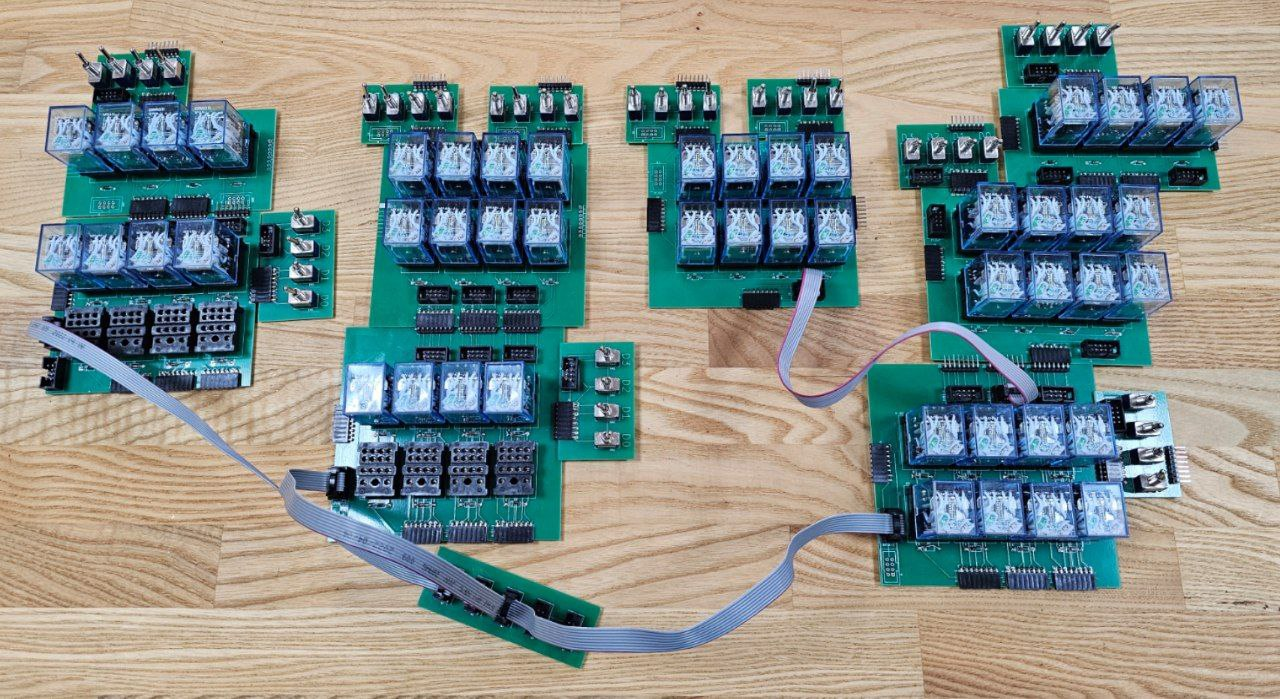
\includegraphics[width=\columnwidth]{photo/calculator.jpg}

Любую из операций можно выполнить так:

\begin{enumerate}
    \item Отключить все управляющие сигналы.
    \item Набрать входные данные для нужной операции.
    \item Подключить выход нужного модуля к регистру тумблером.
    \item Наблюдать результаты вычислений.
    \item Сбросить значение регистра.
\end{enumerate}

